% !TEX TS-program = pdflatex
% !TEX encoding = UTF-8 Unicode

% This is a simple template for a LaTeX document using the "article" class.
% See "book", "report", "letter" for other types of document.

\documentclass[11pt]{article} % use larger type; default would be 10pt

\usepackage[utf8]{inputenc} % set input encoding (not needed with XeLaTeX)

%%% Examples of Article customizations
% These packages are optional, depending whether you want the features they provide.
% See the LaTeX Companion or other references for full information.

%%% PAGE DIMENSIONS
\usepackage{geometry} % to change the page dimensions
\geometry{a4paper} % or letterpaper (US) or a5paper or....
% \geometry{margin=2in} % for example, change the margins to 2 inches all round
% \geometry{landscape} % set up the page for landscape
%   read geometry.pdf for detailed page layout information

\usepackage{graphicx} % support the \includegraphics command and options

% \usepackage[parfill]{parskip} % Activate to begin paragraphs with an empty line rather than an indent

%%% PACKAGES
\usepackage{booktabs} % for much better looking tables
\usepackage{array} % for better arrays (eg matrices) in maths
\usepackage{paralist} % very flexible & customisable lists (eg. enumerate/itemize, etc.)
\usepackage{verbatim} % adds environment for commenting out blocks of text & for better verbatim
\usepackage{subfig} % make it possible to include more than one captioned figure/table in a single float
% These packages are all incorporated in the memoir class to one degree or another...

%%% HEADERS & FOOTERS
\usepackage{fancyhdr} % This should be set AFTER setting up the page geometry
\pagestyle{fancy} % options: empty , plain , fancy
\renewcommand{\headrulewidth}{0pt} % customise the layout...
\lhead{}\chead{}\rhead{}
\lfoot{}\cfoot{\thepage}\rfoot{}

%%% SECTION TITLE APPEARANCE
\usepackage{sectsty}
\allsectionsfont{\sffamily\mdseries\upshape} % (See the fntguide.pdf for font help)
% (This matches ConTeXt defaults)

%%% ToC (table of contents) APPEARANCE
\usepackage[nottoc,notlof,notlot]{tocbibind} % Put the bibliography in the ToC
\usepackage[titles,subfigure]{tocloft} % Alter the style of the Table of Contents
\renewcommand{\cftsecfont}{\rmfamily\mdseries\upshape}
\renewcommand{\cftsecpagefont}{\rmfamily\mdseries\upshape} % No bold!

%%% END Article customizations

%%% The "real" document content comes below...

\title{electricityMap data analyst challenge}
\author{Julie Sainmont}
%\date{} % Activate to display a given date or no date (if empty),
         % otherwise the current date is printed 

\begin{document}
\maketitle

\section{Two electricity zones in Denmark}

Denmark has two electricity zones:
\begin{itemize}
\item The Eastern part of Denmark, covering Zealand with nearby islands and Bornholm, is connected to the synchronous electrical grid of Norway, Sweden and Finland. The hydroelectricity produced by Sweden and Norway provides a stable source of renewable energy that complements the domestic green production of wind energy.
\item The Western part of Denmark is part of the synchronous grid of Continental Europe which is the largest  synchronous electrical grid in the world and includes most of the European Union.
\end{itemize}
We will focus on the Eastern network in this report.

\section{Changes of the carbon footprint of electricity throughout the day}

\begin{figure}[h!]
  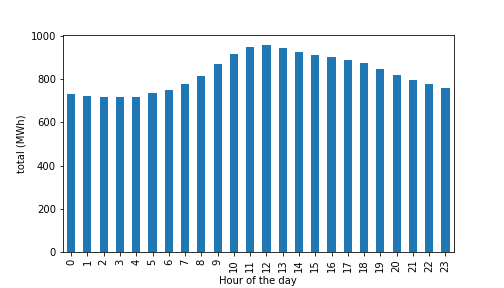
\includegraphics[width=0.8\linewidth]{../outputs/total.png}
  \caption{Energy produced (MWh) throughout the day on average over the year 2020.}
  \label{fig:total_kwh}
\end{figure}
The total energy production varies throughout the day, and is the highest during the business hours, peaking at 1pm (figure \ref{fig:total_kwh}). However to decide when it is the best time to use energy based on minimizing the carbon footprint, we should dive into the different energy sources, their respective carbon emission and their output variations across the day.\\

\begin{figure}[h!]
  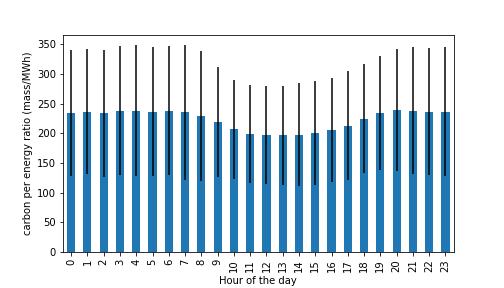
\includegraphics[width=0.8\linewidth]{../outputs/carbon_per_energy_ratio.png}
  \caption{Carbon emitted per energy produced throughout the day on average over the year 2020.}
  \label{fig:co2_kwh}
\end{figure}
 
\begin{figure}[h!]
  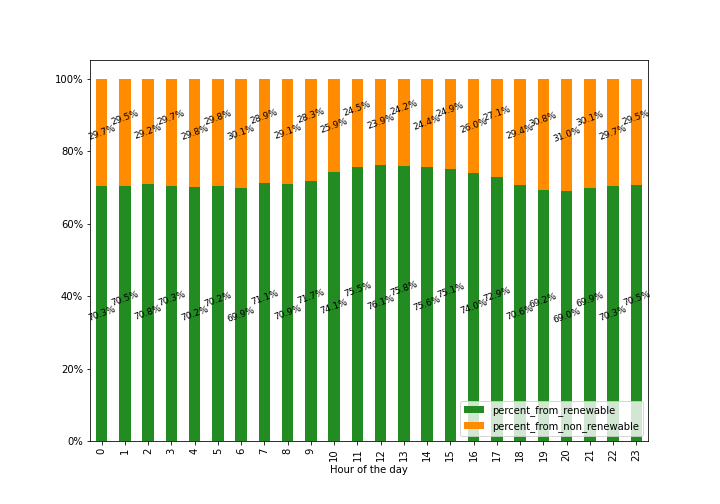
\includegraphics[width=1\linewidth]{../outputs/generated_energy_green_percent.png}
  \caption{Production of renewable and non-renewable energy produced throughout the day on average over the year 2020.}
  \label{fig:per_green}
\end{figure}

\begin{figure}[h!]
  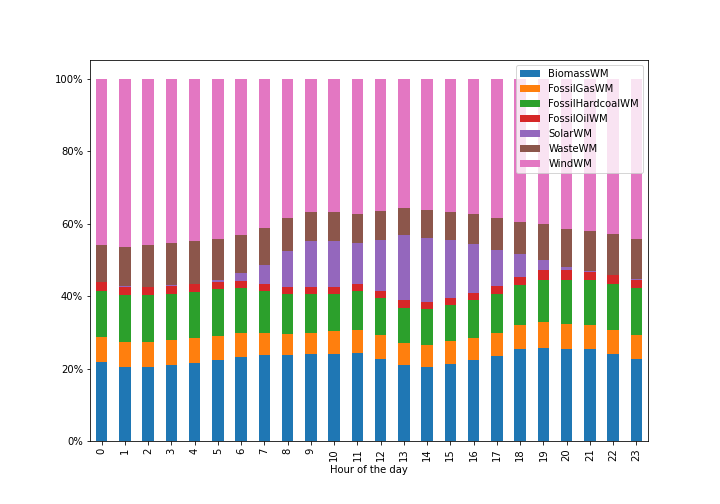
\includegraphics[width=0.9\linewidth]{../outputs/generated_energy_precent_per_sources.png}
  \caption{Production of renewable and non-renewable energy produced throughout the day on average over the year 2020.}
  \label{fig:per_source}
\end{figure}

The energy produced in Eastern Denmark comes from both renewable sources such as biomass, solar and wind; and from large carbon emitting sources such as gas, oil and coal that support the grid when the energy consumption exceeds the production of renewable energy.
When looking at the carbon emissions produced per energy (figure \ref{fig:co2_kwh}), we can see that the time of lowest carbon footprint is during business hours (8am to 5pm), spiking at around 1pm. The average variation of carbon emission throughout of the day is close to 20\%. It is therefore on average better to consume energy during the peak energy production hours of the day. This finding is supported by the average fraction of energy contribution from renewable and non-renewable sources (figure \ref{fig:per_green}).\\

To understand this otherwise counter-intuitive finding, we can look at the production of renewable energy sources throughout the day (see appendix \ref{app:renewable} for details), and see that although the average wind production is constant through the day, the biomass, and in particular the solar energy sources peak during the day. When looking at the fraction of the total energy production from the different sources, we can see that it is the larger solar contribution to the renewable sources of energy during the middle of the day that brings the total fraction of renewable energy output to its highest level (figure \ref{fig:per_source}).

\clearpage\newpage
\section{Utilizing the data to decide when to charge at the greenest time}
If the wind and solar energy are the main contributors to the renewable electricity, is it every day that it is better to use energy during the middle of the day throughout the seasons? After all, '\textit{the wind doesn't always blow and the sun doesn't always shine}' (\ref{app:time_serie}), how can we know when it is the best time to charge the batteries of our electrical cars to minimise our carbon footprint ?  \\

The electricityMap can provide your members with an estimate of the best time to use electricity in the next 24h to empower you to effectively reduce your energy footprint. With this prediction, your members will be able to choose when to plug or schedule the charger to start recharging their cars at the optimal time of the day. We also offer to track your emissions so you can track and visualise the impact of your efforts of their emissions.


%---  Appendix
\clearpage\newpage
\appendix

\section{Renewable average production over the day}\label{app:renewable}
% Solar
\begin{figure}[h!]
  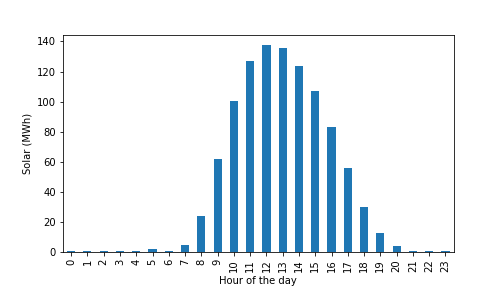
\includegraphics[width=0.8\linewidth]{../outputs/Solar.png}
  \caption{Solar energy produced throughout the day in average over the year 2020.}
  \label{fig:solar_kwh}
\end{figure}
% Biomass
\begin{figure}[h!]
  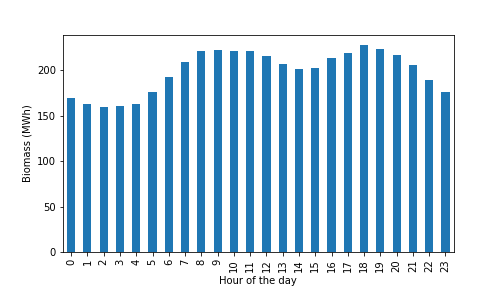
\includegraphics[width=0.8\linewidth]{../outputs/Biomass.png}
  \caption{Biomass energy produced throughout the day in average over the year 2020.}
  \label{fig:biomass_kwh}
\end{figure}
% Wind
\begin{figure}[h!]
  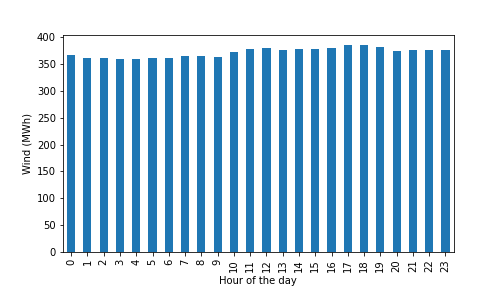
\includegraphics[width=0.8\linewidth]{../outputs/Wind.png}
  \caption{Wind energy produced throughout the day in average over the year 2020.}
  \label{fig:wind_kwh}
\end{figure}


\clearpage\newpage
\section{Non-renewable averable production over the day}\label{app:non_renewable}
% Gas
\begin{figure}[h!]
  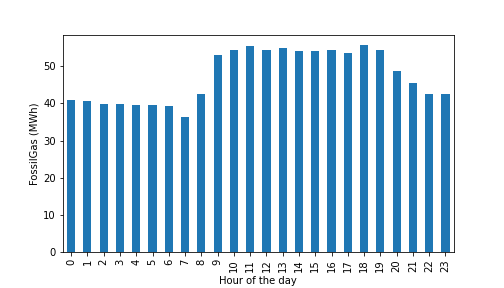
\includegraphics[width=0.8\linewidth]{../outputs/FossilGas.png}
  \caption{Fossil gas energy produced throughout the day in average over the year 2020.}
  \label{fig:gas_kwh}
\end{figure}
% coal
\begin{figure}[h!]
  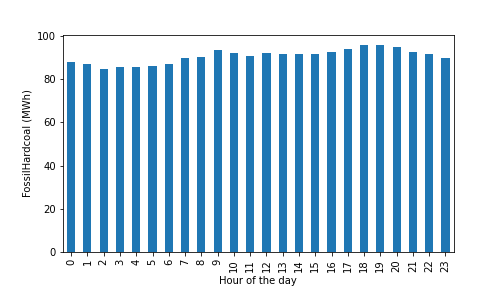
\includegraphics[width=0.8\linewidth]{../outputs/FossilHardcoal.png}
  \caption{Fossil hard coal energy produced throughout the day in average over the year 2020.}
  \label{fig:coal_kwh}
\end{figure}
% Oil
\begin{figure}[h!]
  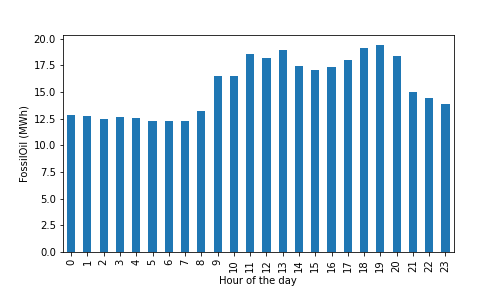
\includegraphics[width=0.8\linewidth]{../outputs/FossilOil.png}
  \caption{Fossil Oil energy produced throughout the day in average over the year 2020.}
  \label{fig:oil_kwh}
\end{figure}


\clearpage\newpage
\section{Time serie of the 2020 year energy production}\label{app:time_serie}
\begin{figure}[h!]
  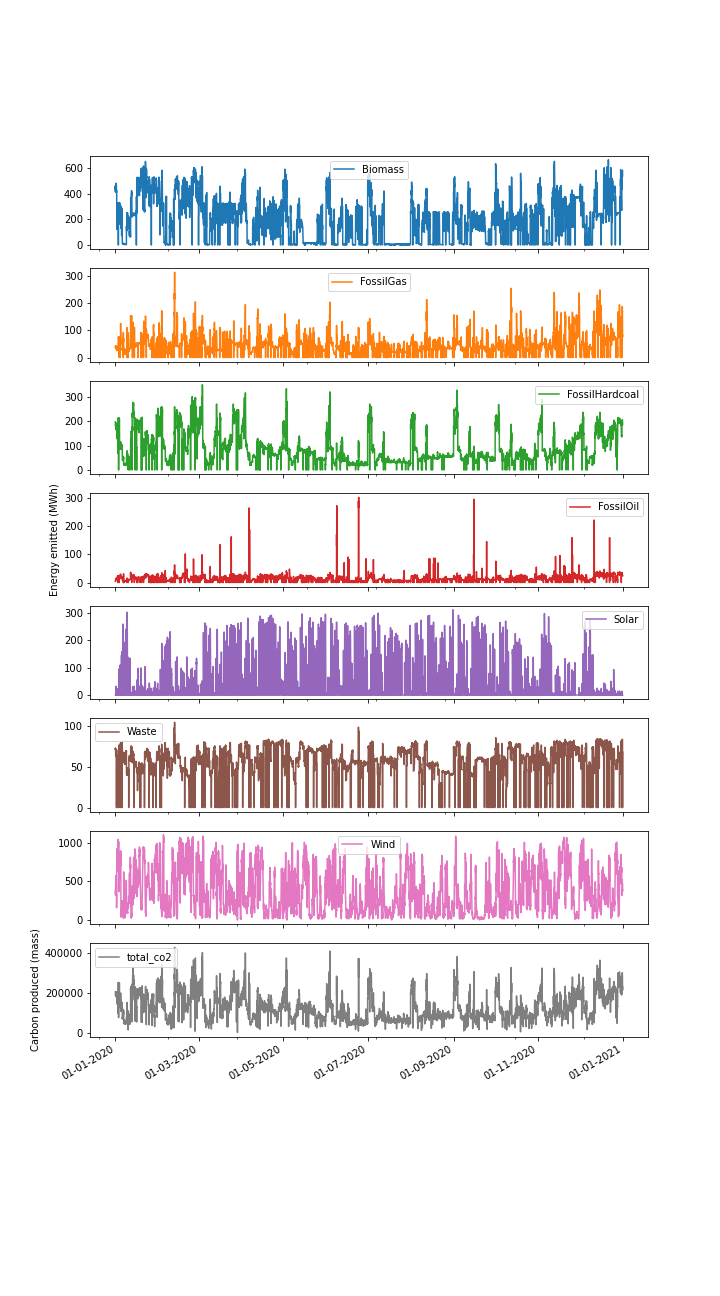
\includegraphics[width=0.7\linewidth]{../outputs/energy_production_time_serie.png}
  \caption{Time serie visualization of the energy produced in Eastern Denmark and the carbon emission over the year 2020. The top 6 graphs shows the energy produced from the different sources, and is expressed in kWh, while the bottom graph shows the carbon emission and is expressed in gram of CO$_2$}
  \label{fig:time_series}
\end{figure}


\end{document}
